\clearpage
\chapter{Introduction}


Generative Artificial Intelligence (AI) is a rapidly advancing 
branch of AI that, in recent years, has made 
tremendous progress, largely due to the widespread adoption of 
deep learning techniques. Generative models 
are now powerful deep learning architectures capable of producing 
highly realistic text, images, and even video content.


The famous Turing Test is frequently referenced in this context. 
In this test, a human judge had to determine whether they were 
communicating with another human or with a machine. This milestone 
was already surpassed in 2014, with early systems such as Eugene Goostman 
\cite{warwick2016turing}.


Today, it is widely accepted that much of the content generated by 
generative models is indistinguishable from human-produced material
and indeed, for humans, \textbf{this distinction is increasingly difficult 
to make}.


The introduction of the Transformer architecture in 2017 
\cite{vaswani2017attention} revolutionized the field 
and led to the development of Large Language Models (LLMs), 
which quickly became part of everyday life. This wave began 
with the public availability of GPT-3 \cite{brown2020language} in June 2020 
\cite{brown2020language}, followed by a growing ecosystem of 
LLMs including GPT-4 \cite{openai2023gpt4}, PaLM 
\cite{chowdhery2022palm}, LLaMA \cite{touvron2023llama}, 
Claude \cite{anthropic2023claude}, and Mistral \cite{jiang2023mistral}.

Generative AI, however, is not limited to natural language 
processing. It has also enabled powerful models for image 
generation, such as Stable Diffusion \cite{rombach2022high}, 
and more recently for video 
synthesis, with systems like Veo-3 \cite{google2024veo}.


Although the usefulness and extraordinary capabilities of these 
tools are undeniable, there are many scenarios in which it becomes 
necessary to have user-friendly tools to detect whether text, images, 
or videos were generated by an AI.

The present work pursues a more modest, yet equally important objective: the
\textbf{detecting artificially generated source code} produced by code generation 
models such as OpenAI Codex \cite{chen2021codex}, GPT-4 \cite{openai2023gpt4}, 
and Code LLaMA \cite{roziere2023code}.


While natural language detectors are well-established and widely 
studied in scientific literature, the detection of AI-generated code 
remains a far less consolidated and more recent research area. 
The contribution of this work is to \textbf{analyze the most relevant 
scientific advancements} made in the past year, which are often fragmented and 
inconsistent due to the unique challenges involved in distinguishing 
machine-generated code, a task that is arguably more complex than natural 
text detection.




\clearpage
\section{Historical Overview of Code Generation by LLMs}

The history of code generation can be explored from several 
perspectives. 

\subsection{Natural Language Processing} %%%%%%%%%%%%%%%%%%%%%%%%%%%%%
One possible starting point possible perspective for 
analysing the evolution of code generation is to trace
the development of Natural Language Processing (NLP), 
the field that studies how machines process and interact 
with human language. NLP comprises two major subdomains: 
Natural Language Understanding (NLU), which focuses on a 
machine's ability to interpret and "understand" human language, 
and Natural Language Generation (NLG), which concerns the 
generation of natural-sounding text.

This distinction is particularly relevant because 
the technologies currently used for code generation 
are essentially the same as those employed for natural 
language generation. In fact, Transformer-based models 
trained on source code data approach code generation in 
the same way they would handle natural text generation 
by predicting sequences of tokens in context using learned 
statistical patterns \cite{vaswani2017attention}.

From this point of view, the starting point can be traced back to 1943, 
during World War II, with the invention of Colossus, one of the first digital 
electronic computers, developed to analyse encrypted communications from the 
German military

In parallel, the discipline of Natural Language Processing 
(NLP) began to take shape as early as the 1940s, culminating 
in the 1954 Georgetown experiment the first public demonstration 
of machine translation. Another milestone came in 1966 with the 
creation of ELIZA \cite{weizenbaum1966eliza}, considered the first 
chatbot in history, which simulated the behaviour of a psychotherapist 
using pattern-matching rules.

During the 1970s and 1980s, symbolic approaches to NLP became popular. 
These early attempts aimed to enable machines to “understand” language 
through manually encoded rules and logic-based systems. In the 1990s, 
the importance of statistical methods became evident, marking a shift 
from rule-based to probabilistic models for language processing.

In 2006 Google launched its now ubiquitous Google 
Translate service. The following decade saw the rise of voice-based 
assistants: Apple’s Siri (2011), Microsoft’s Cortana (2014), 
Amazon’s Alexa (2014), and Google Assistant (2016).

A major breakthrough came with the introduction of distributed word 
representations, especially word2vec \cite{mikolov2013efficient} and 
GloVe \cite{pennington2014glove}, published in 2013 and 2014 respectively. 
These methods enabled dense vector representations that captured semantic 
relationships between words in large corpora.

The most significant leap, however, occurred in 2017 with the publication 
of the now seminal paper “Attention is All You Need” 
\cite{vaswani2017attention}, which introduced the Transformer 
architecture. This architecture remains the dominant framework in 
NLP and underpins nearly all modern LLMs. Transformers enabled major 
advances in tasks such as text generation, machine translation, 
question answering, text summarization and, more recently, code 
generation.

The first LLMs capable of code generation began to appear around 
2019–2020, notably with the release of GPT-2 \cite{radford2019language}. 
In 2021, OpenAI released Codex \cite{chen2021codex}, a GPT-3 \cite{brown2020language} derivative 
trained specifically for code generation and explanation, which was
later integrated into GitHub Copilot.

Between 2022 and 2024, a wave of new LLMs for code generation was 
released, including CodeT5 \cite{wang2021codet5}, CodeGen 
\cite{nijkamp2022codegen}, CodeGeeX \cite{zeng2022codegeex}, 
and Code LLaMA \cite{roziere2023code}.


\subsection{Code Generator} %%%%%%%%%%%%%%%%%%%%%%%%%%%%%
\label{sec:Code_Generator}
Another possible point of view is the one focused on code 
generation itself. This is not a  completely new concept: 
it dates back to 1957 with Fortran. Fortran is both a 
programming language with an integrated compiler, developed by IBM. 
A compiler can be seen as a code generation tool, since it 
translates source code into machine code, the only “language” 
truly “understandable” by a computer \cite{backus1957fortran}.

Compilers have a long history and have been continuously 
improved over time, but they are not the only tools for code 
generation. Already in 1976, the concept of intelligent editors 
emerged with Emacs, thanks to its support for custom macros 
\cite{stallman1981emacs}. Later, in 1996, IntelliSense 
introduced symbolic completion, namely the ability of the IDE 
to suggest code based on the context and the symbols already present.

In 1999, with XSLT, one of the first standardized tools for 
automatic transformation between markup languages was introduced 
\cite{xslt1999}. During the same years, the work of Zelle\cite{zelle1996learning}
and  Mooney\cite{mooney1997nlidb} (1996–1999) 
proposed methods based on Natural Language 
processing to generate database queries from natural language 
expressions.

At the same time, template-engine-based tools  for server-side 
spread, such as Jinja2 (2005)\cite{jinja2docs} 
and Mako (2006)\cite{makoengine}, 
which allowed the generation of 
dynamic code by combining data with predefined structures. 

In 2017, with research on AST-guided code generation, LSTM 
models began to be used to generate code in a more structured 
way, guided by the syntax of the programming language 
\cite{yin2017syntactic}.

Finally, in 2021, with GitHub Copilot, one of the most advanced 
code completion tools was introduced: so efficient that it is 
capable of generating entire code sections from simple textual 
prompts, thanks to the use of generative AI models based on 
Transformer architectures \cite{chen2021codex}.




\subsection{LLMs code oriented} %%%%%%%%%%%%%%%%%%%%%%%%%%%%%
Another possible starting point is from the publication of the 
paper \textit{Attention Is All You Need} in 2017, which 
introduced the Transformer architecture \cite{vaswani2017attention}
and, enabled the widespread development of
Large Language Models (LLMs). 
It should be noted that the first LLMs were typically designed 
to analyse and generate only natural language text, so not all LLMs 
were capable of generating code, or at least of generating syntactically 
correct or functional code.

In 2018, two foundational models were introduced: BERT 
\cite{devlin2019bert}, an encoder-only architecture 
designed to generate dense semantic representations of 
natural language, and GPT-1 \cite{radford2018improving}, 
a decoder-only model capable of generating coherent text. 
Those models were not yet able to generate code, but they have been 
an important baseline for future code-oriented models.

In fact in 2019, OpenAI released GPT-2 \cite{radford2019language}, 
a more powerful decoder-only model capable of producing much 
more convincing text compared to GPT-1. Although GPT-2 was 
not specifically trained to generate code, its training 
corpus included code snippets. In the same year, 
TabNine, a popular code completion extension for several IDEs, 
replaced its n-gram-based next-token prediction with a version 
of GPT-2 fine-tuned on source code \cite{tabnine2019}.

Also in 2019, Microsoft Research and GitHub introduced the 
CodeSearchNet dataset \cite{husain2019codesearchnet}, a 
multilingual code dataset and one of the first large-scale 
corpora usable to train Transformers for code generation tasks.

In 2020, Microsoft Research released CodeBERT 
\cite{feng2020codebert} \textit{(based on BERT)}, 
trained on both natural 
language and code using the CodeSearchNet dataset. 
CodeBERT is designed for tasks such as code search 
and code summarization. While it does not generate code, 
it is an encoder-only model capable of deeply understanding 
the structure and semantics of source code. Through 
CodeBERT is possible producing rich 
and dense representations suitable for downstream tasks like 
classification, or for use as input to decoders in generative 
pipelines.

In 2021, several LLMs capable of generating realistic and 
reliable code were introduced. OpenAI published Codex 
\cite{chen2021codex}, a GPT-3 \cite{brown2020language} derivative fine-tuned on 
source code from the GitHub Code dataset. In the same paper 
OpenAI introduced the HumanEval benchmark, designed to assess the 
performance of Codex \cite{chen2021codex} on programming problems 
\textit{(and in future all LLMs code oriented)}.
On HumanEval, Codex (12B) was able to solve 28.8\% 
of the problems on the 
first attempt, significantly outperforming all previous 
models on code generation.

Codex \cite{chen2021codex} sparked widespread interest in the use of LLMs 
for code generation, indeed in the same year is released 
GitHub Copilot, powered by Codex \cite{chen2021codex}.

In the same year, 
many additional datasets were 
published, including MBPP (Mostly Basic Python Problems) 
\cite{austin2021program}, the APPS dataset \cite{hendrycks2021measuring}, 
and CodeXGLUE \cite{lu2021codexglue}.

In December 2021, Salesforce AI Research released CodeT5 
\cite{wang2021codet5}, an open-source encoder-decoder 
model that, unlike Codex \cite{chen2021codex}, supports a wider variety of 
code-related tasks. Thanks to task-specific training strategies, 
CodeT5 proved to be highly versatile, supporting code 
summarization, generation, and translation.

In 2022, Google introduced AlphaCode \cite{li2022competition}, 
achieving a performance in the top 54.3 percentile on 
competitive programming tasks on Codeforces. In the same 
year, PolyCoder \cite{xu2022systematic}, a decoder-only 
model trained solely on 249 GB of source code, was also 
released as an open-source alternative. 

In 2023, GPT-4 \cite{openai2023gpt4} (although not 
exclusively trained for code generation)  
achieved an 80\% success rate on HumanEval. 
Claude 3 by Anthropic reportedly reached 85\%, 
and Meta’s open-source model Code LLaMA 
\cite{roziere2023code} scored 57\%.

In 2024, Google introduced Gemini \cite{AlphaCode_2}, 
which, when integrated into an inspired AlphaCode framework, 
reached performance within the top 15\% of coding competition 
participants.



\begin{figure}[ht]
    \centering
    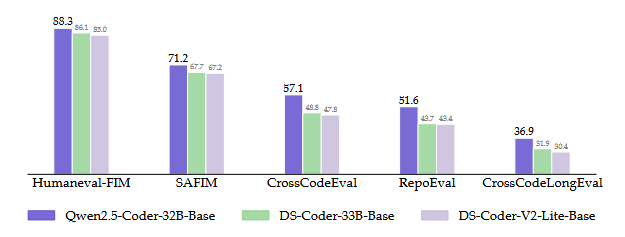
\includegraphics[width=0.8\textwidth]{img/1/image.png}
    \caption{The code completion performance of competitive models on five benchmarks,
Humaneval-FIM, SAFIM, CrossCodeEval, RepoEval, CrossCodeLongEval from \cite{hui2024qwen2}.}
    \label{fig:LLM-coder-examples}
\end{figure}
\clearpage
\section{Motivations Behind LLM-Generated Code Detection}
Although it may seem exaggerated to begin the historical 
overview of code generation 
\hyperref[sec:Code_Generator]{Section 1.1.2} with compilers, 
this choice aims to emphasize that the present work does not 
seek to demonize the contribution or usefulness of code 
generation tools. It is undeniable that such tools are 
extremely valuable in both professional software development, 
accelerating simpler phases of implementation, and 
in educational contexts, where they can serve as 
useful assistants for learning how to write code.

Nevertheless, it is equally clear that is raising 
the need, in certain contexts 
and for specific reasons, to limit or discourage 
the use of highly advanced tools for code autocompletion 
or generation.

\vspace{1\baselineskip}
\noindent

One important reason concerns \textbf{academic and 
professional integrity}: the undeclared use of 
LLMs in evaluation contexts makes the assessment 
process highly problematic. Students, for example, 
may complete assignments or even exams using LLMs 
without contributing meaningfully to the generated 
code, potentially impairing their learning of 
fundamental programming concepts 
(getting the most out with the least effort). Similarly, 
during a technical interview, a candidate might 
rely on a tool like AlphaCode 2 to generate solutions 
to proposed problems.
This is the main topic of
\textit{"The Impact of Large Language Models on 
Programming Education…"} \cite{Jost2024LLM}
in which is demonstrated that a widespread use of 
LLMs code generator has negatively affects 
over students' capability.

Figure~\ref{fig:scatterplot} illustrates 
possible correlation between final grade and the
use of LLM. We can observe that an increase 
in LLM usage tends to correlate with lower 
average student grades, although it is not a 
decisive factor in determining the final score.

%Several studies raise concerns about these issues, 
%including: 
%Demirok and Kutlu\ cite{demirok2025aigcodeset}, 
%Xu and Sheng \cite{xu2025codevision}, 
%Ye et al. \cite{ye2025uncovering}, 
%Orel, Azizov, and Nakov \cite{orel2025codetm4}, 
%Yang et al. \cite{yang2023zeroshot}, 
%Nguyen et al. \cite{nguyen2023snippet}, 
%Hoq et al. \cite{hoq2023detecting}, 
%Paek and Mohan \cite{paek2025java}, 
%Bulla et al. \cite{bulla2024excode}, 
%Pham et al. \cite{pham2023magecode}, 
%and Park et al. \cite{park2025paraphrased}.

\vspace{1\baselineskip}
\noindent

Another critical issue lies in the way LLMs generate code. 
Since these models are trained on massive corpora, 
evaluating the security and efficiency of the generated 
code is nearly impossible. The output may be 
\textbf{vulnerable or inefficient} 
due to subtle flaws that are hard to detect, especially 
when the code appears well-formatted and logically 
structured. 
This happens to overreliance on 
commonly seen patterns in the training corpus rather 
than more appropriate niche solutions.
The security issues are highlighted by the study
\textit{”Do Users Write More Insecure Code with AI Assistants?”} 
\cite{perry2022users}. This study shows a decrease in
code security simply by using an AI assistant instead of
traditional programming.

%Relevant studies that address this concern include: 
%Suh et al. \cite{suh2024empirical}, 
%Demirok and Kutlu \cite{demirok2025aigcodeset}, 
%Shi et al. \cite{shi2024between}, 
%Ye et al. \cite{ye2025uncovering}, 
%Rahman et al. \cite{rahman2024claude}, 
%Bulla et al. \cite{bulla2024excode}, 
%Orel et al. \cite{orel2025codetm4}, 
%Yang et al. \cite{yang2023zeroshot}, 
%Xu et al. \cite{xu2023perplexity}, 
%and Nguyen et al. \cite{nguyen2023snippet}.

\vspace{1\baselineskip}
\noindent

\textbf{Intellectual property} is yet another motivation 
for detecting LLM-generated code, a general problem 
in generative AI. This is not limited to the origin 
of training data but also concerns the risk that an 
LLM may reproduce copyrighted code, posing 
significant legal risks to software companies 
that could unknowingly integrate such code into 
their products.
This issue is not an exaggerated concern, 
it's a tangible risk \cite{DoeVGitHub2024}.

%This issue has been raised in several studies, 
%including Suh et al. \cite{suh2024empirical}, 
%Yang et al. \cite{yang2023zeroshot}, 
%Nguyen et al. \cite{nguyen2023snippet}, 
%Paek and Mohan \cite{paek2025java}, 
%Park et al. \cite{park2025paraphrased}, 
%and Rahman et al. \cite{rahman2024claude}.

\vspace{1\baselineskip}
\noindent

The least important reason, 
which directly 
concerns the development of code-oriented 
LLMs themselves, is the need to distinguish 
machine-generated code in training datasets. 
If a model is trained on LLMs' code we might run into
a general LLM code oriented \textbf{Model Collapse}. 
Indeed, training LLM on LLMs' code serves to deteriorate the 
output diversity and adaptability to real-world scenarios.
This feedback loop issue is addressed for example in 
\textit{"The curse of recursion…"} 
\cite{shumailov2023curse}.
If no method exists to detect such code, the 
datasets used for training future models would 
have to be limited to code written before the 
widespread availability of LLMs, in order to 
avoid contamination. This would result in 
code generation models being trained on 
increasingly outdated data. 


% This issue is notably highlighted by Orel, 
% Orel, Azizov, and Nakov~\cite{orel2025codetm4}.

%%% Figura studenti
\begin{figure}[H]
    \centering
    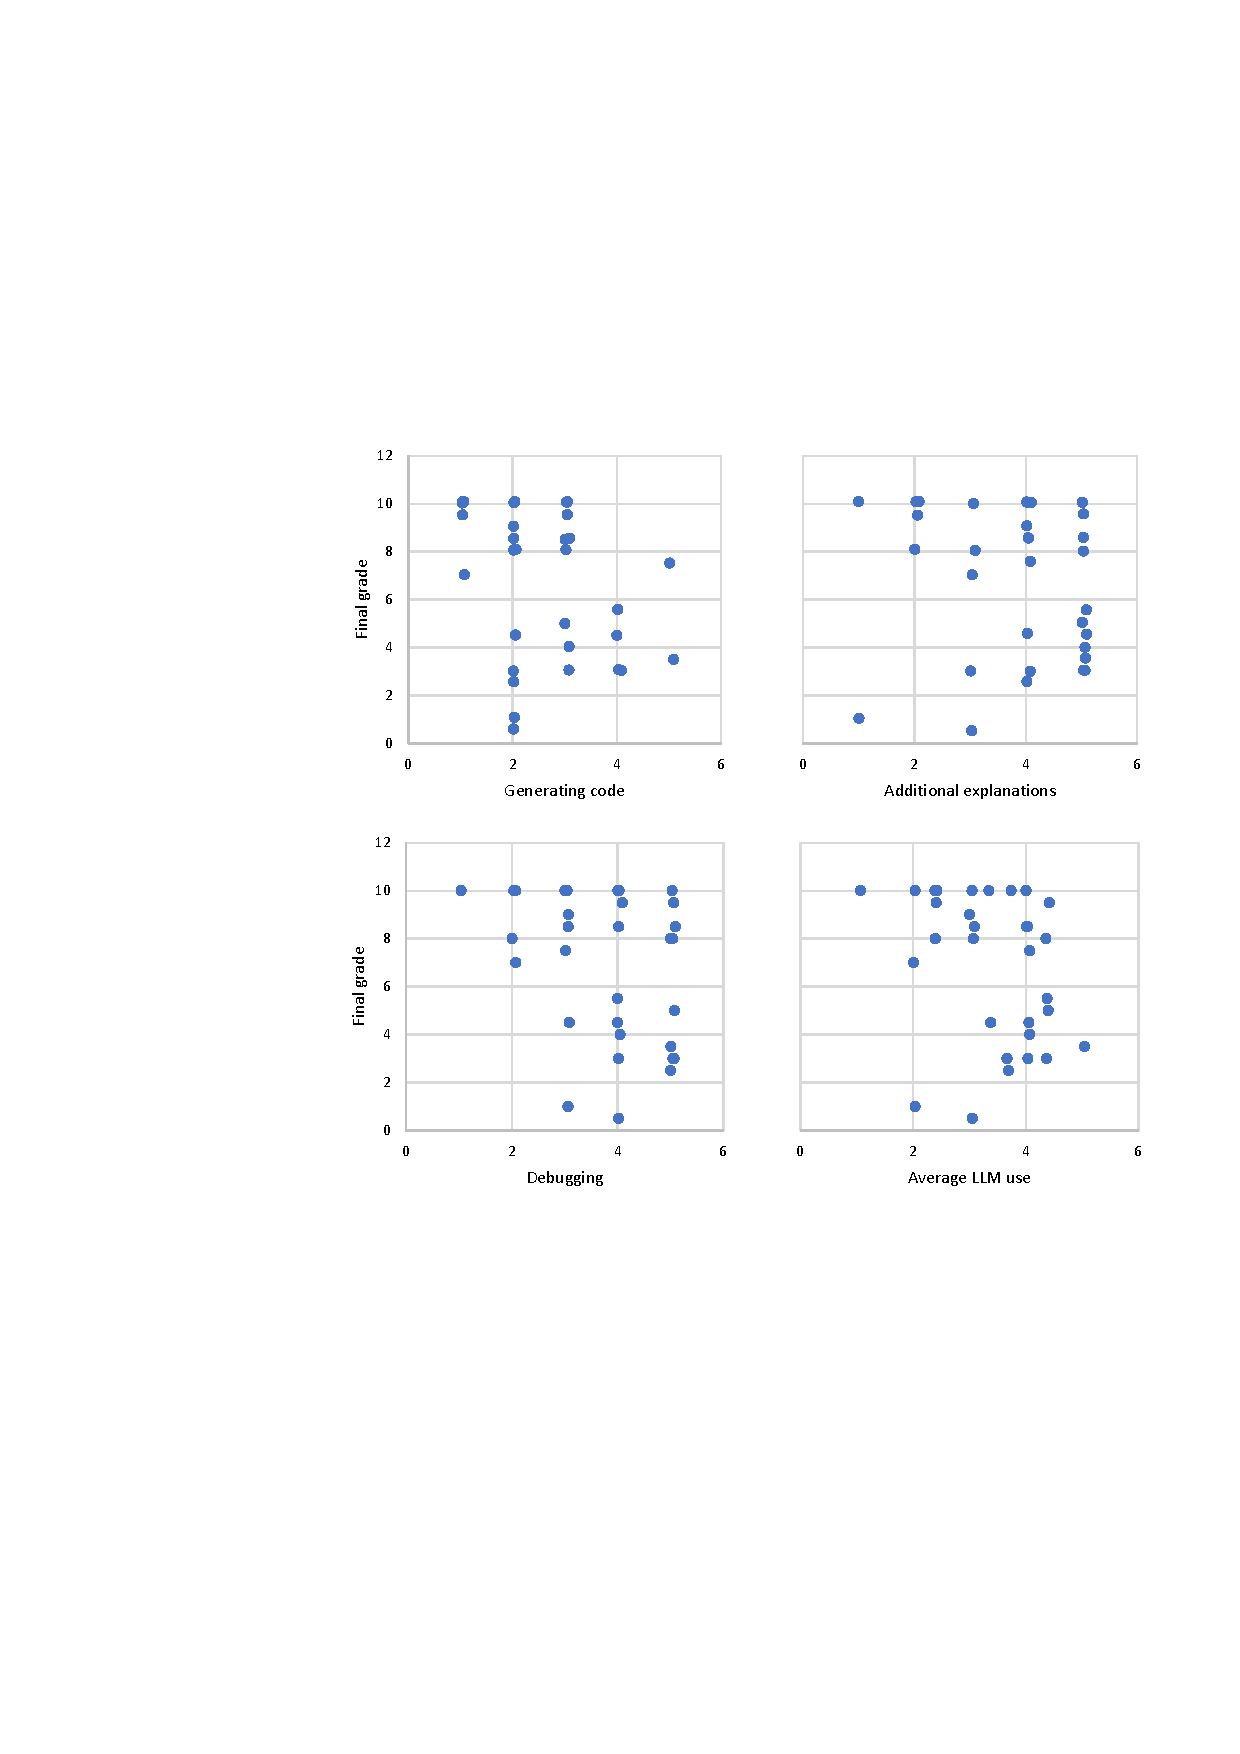
\includegraphics[width=0.9\textwidth]{img/1/scatterplot.pdf}
    \caption{Scatter plot from the paper 
        \emph{The Impact of Large Language 
        Models on Programming Education and 
        Student Learning Outcomes}, 
        illustrating the relationship between 
        LLM usage and students' final performance.}

    \label{fig:scatterplot}
\end{figure}
\clearpage
\section{Challenges in LLM-Generated Code Detection}
\label{sec:Challenges in LLM-Generated Code Detection}
The detection of short texts generated by LLMs remains 
a challenging task. While partial solutions have been 
proposed, the problem cannot yet be considered fully 
resolved. Nonetheless, it is widely acknowledged that 
detection tools achieve strong performance when applied 
to moderately sized texts (longer than just a few lines).

A well-known example is \textbf{DetectGPT}
\cite{mitchell2023detectgpt}, a 
zero-shot method that does not require training a 
separate classifier but instead relies on an 
auxiliary LLM to assess whether a given passage is 
likely machine-generated. 
DetectGPT is often regarded as the state-of-the-art 
among open-source methods for AI-generated text detection.

%Eliminato per rientrare in una pagina
%However, recent studies have shown that even minimal 
%perturbations to LLM-generated outputs can significantly 
%reduce detection AUROC, in some cases down to 
%42\% \cite{krishna2023paraphrasing}. These findings 
%highlight that detection performance is highly 
%sensitive to surface-level edits.

In addition to open-source methods, commercial 
solutions such as \textbf{GPTZero} \cite{GPTZeroMethodology2023}
have gained 
popularity. GPTZero can be accessed via a web 
interface and combines language-model-based heuristics 
with machine learning classifiers. While it is 
effective in many cases, it is not infallible. 
For example, GPTZero has been reported to mistakenly 
flag texts written by non-native speakers, 
whose lexical variety may be lower, as AI-generated.

Even the creators of GPTZero explicitly state 
that a positive detection should not be taken as 
conclusive proof, but rather as a probabilistic 
signal or indicator.

\vspace{1\baselineskip}
\noindent

As stated in several papers analysed in this work, 
such as \textit{Uncovering LLM-Generated Code: A 
Zero-Shot Synthetic Code Detector via Code Rewriting 
\cite{ye2023uncovering}}, \textbf{methods designed for 
detecting natural language text are largely 
ineffective when applied to code}. The causes of 
this limitation are primarily related to the 
structural and syntactic properties of programming 
languages. 

Unlike natural language, where the same idea 
can be expressed using a vast variety of words 
and syntactic structures, source code is governed 
by strict and formal grammar rules. As a result, 
many tokens must appear in a specific and rigid 
order. Consequently, techniques based on lexical 
probability, such as those used by DetectGPT, 
tend to fail when applied to code, as they cannot 
meaningfully capture the constrained nature of 
programming syntax.

Moreover, many natural language detectors 
rely on input perturbation to assess sensitivity 
or likelihood distributions, a process that is 
significantly more difficult to perform on source 
code without introducing semantic or syntactic errors.

A further practical limitation is the lack of 
publicly available datasets specifically designed 
for training code-based LLM detectors. While large 
and well-established code corpora do exist, 
researchers who aim to train classification models 
for code detection often have to construct their 
own datasets, with all the associated challenges 
in terms of bias, coverage, and quality assurance.

These issues have contributed to a significant 
gap in the literature: unlike DetectGPT, which is 
widely recognized for natural language detection, 
there is no single, consolidated approach for 
LLM-generated code detection. Instead, the field 
is characterized by a proliferation of parallel 
methods, often employing fundamentally different 
techniques and evaluation protocols.



\begin{figure}[H]
    \centering
    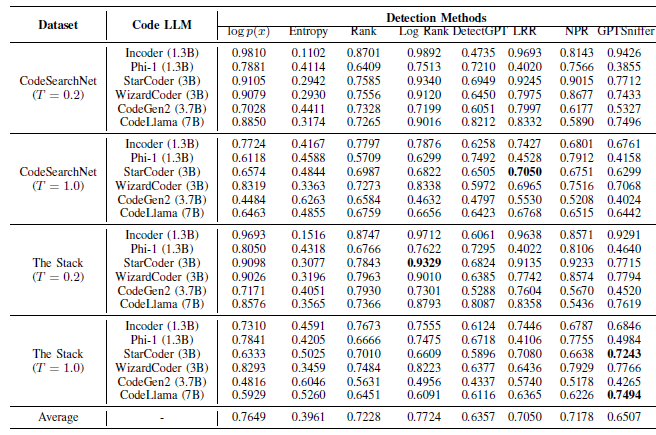
\includegraphics[width=0.9\textwidth]{img/1/Berween.png}
    \caption{Performance (AUROC) of various detection methods from \cite{shi2024between}.}

    \label{fig:Performance (AUROC) of various detection methods}
\end{figure}
\clearpage

\section{Thesis Objectives}
This thesis aims to pursue a structured series 
of objectives, each forming a necessary foundation 
for the subsequent stage of the project.

The overarching goal is to \textbf{develop a software 
tool capable of reliably distinguishing source 
code written by humans from that generated by 
Large Language Models} (LLMs). Given the lack of 
standardization in the current literature, this 
project first seeks to \textbf{establish a fair and 
reproducible evaluation framework}.

The initial task involves \textbf{selecting} a 
sympathetic and representative \textbf{dataset} 
that can serve both for retraining detection 
models and for evaluating their performance 
consistently. A comparative analysis of 
current scientific literature datasets 
will be conducted, taking into 
account objective criteria such as class 
balance, diversity of programming languages, 
code length variability, and feature distribution. 
The selected dataset will play a central role in 
ensuring that all subsequent experiments are 
comparable and grounded on a common basis.

Once the dataset is established, the next 
phase consists in \textbf{collecting and systematically 
evaluating the various detection models 
suggested in recent literature}. These models 
will be executed on the selected dataset 
using consistent and comparable metrics in 
order to allow for a meaningful comparison. 
Special attention will be given to 
understanding the assumptions and limitations 
of each model. 
For instance, we will examine 
which datasets were originally used for training, 
which evaluation metrics are most informative 
in this context, the computational requirements 
of each method, and the specific scenarios in 
which they demonstrate optimal or suboptimal performance.
In this phase, it will also be possible to 
identify the underlying reasons why certain 
models outperform others. 

Following this benchmarking effort, the 
most promising method will be selected for 
further investigation. At this stage, will be
proposed enhancements aimed at improving accuracy, 
robustness, or efficiency. These improvements 
must be tailored to the nature of the selected 
model.

The final phase of the project will focus on 
the development of a usable and \textbf{user-friendly 
software interface}, which allows end users 
to apply the selected detection model with 
minimal technical effort. The interface may 
include customizable parameters such as 
confidence thresholds or model options, 
depending on the characteristics of the 
adopted approach. Particular care will be 
taken to ensure that the tool is accessible 
and adaptable, so that it can be employed in 
diverse real-world scenarios, from academic 
integrity enforcement to software development auditing.
Ultimately, this thesis intends to contribute 
both a rigorous comparative study and a 
practical, operational tool, filling a 
current gap in the literature and paving 
the way for future research and application 
in this emerging area
